\documentclass{article}
\usepackage{graphicx}
\usepackage{booktabs}
\usepackage{color, colortbl}
\definecolor{Gray}{gray}{0.9}
\definecolor{LightCyan}{rgb}{0.88,1,1}
\usepackage[first=0,last=9]{lcg}

\begin{document}

    \title{Freelancing Management System \\
    \textbf{FMS}}
    \author{\textit{The Team --- Yaser, Umar, Taha and Boda}}
    \date{March 25, 2017}
\maketitle

\begin{figure}[ht!]
\centering
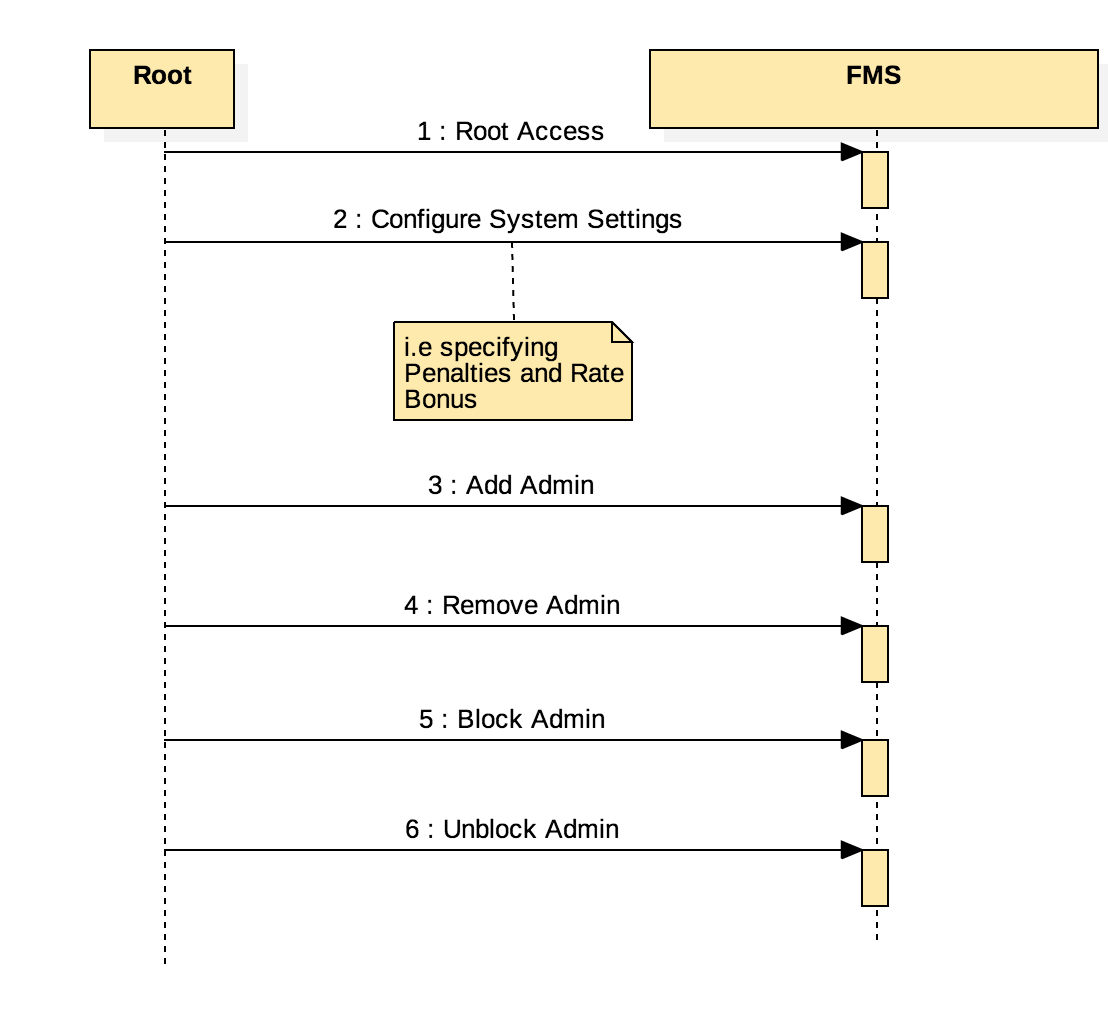
\includegraphics[width=128mm]{SystemSequanceDiagram_Root.png}
\caption{System Sequence Diagram of the \textit{Root}}
\end{figure}

\newpage
\tableofcontents
\newpage



\section{System Description}
  \hspace{0.5cm} This is a \textit{Freelancing Management System}, a system which
  allows \textit{Customers } and \textit{Freelancers} to find
  one--another easily. It manages the processes from finding workers,
  verifying them, engaging, paying up to rating.
  \hspace{0.3cm}Let us take you on an interesting tour into the
  \textit{system actors}, every one of them sees the system differently
  according to their role.

\section{System Actors}
\subsection{Root}
\hspace{0.5cm} \textit{The Root} is the owner of the system. He is the one
who set it up for the first time with a special root access from him.
The Root also specifies the system settings like penalties,
bonuses on the rate and ratio of the profit on each Employer-Freelancer deal. \\
Besides, He add \textit{Admins} to manage the system.









\subsection{Admin}
\hspace{0.5cm} \textit{Admins} are the managers of the system. They have
\textit{The managers access} over the hole system, they can \textit{delete}
or \textit{ban} any consumer account. \\
Also, They can view some Statistics like the number of the Employers and
Freelancer. They can \textit{Receive} and \textit{Reply Complaints} of the
consumers as well. \\Admins can view reports about the system
 i.e \textit{economic}, \textit{consumers}, \textit{blocked}, ...   reports.

\subsection{Freelancer}
\hspace{0.5cm} \textit{Freelancers} are the workers of the system.
Every one them have an \textit{Profile} where he can share his experience,
and work examples. His \textit{Profile} contains enough information
so that the Employer can decide wherever he is going to invest in that
\textit{freelancer} or not.
There is a \textit{Rate} in the \textit{Freelancers Profile} is computed
with very accurate algorithms based on the \textit{Employers Feedback}
and how commitment is the Freelancer!
\textit{Freelancer} are paid per hour, and it is in the \textit{profile}.
A \textit{Freelancer} can review the \textit{Employers' Profiles} and
their \textit{Tasks} which they can apply for it and make special offers
for the \textit{Employers}.


\subsection{Employer}
\hspace{0.5cm} \textit{Employer} are the stockholders. They also have
their \textit{profiles}. An \textit{Employer} can create a \textit{Task} or
\textit{a list of tasks} seen  by interested \textit{Freelancers}.
Then the \textit{Employer} can choose the best \textit{Freelancer} among who
applied. Once the \textit{Employer} accepts the \textit{offer}
the money is \textit{withdrawn} from his account to the pending state in
the system. After the \textit{task} is finished, the \textit{Employer} can
\textit{rate} and \textit{feedback} the \textit{freelancer},
and sure the freelancer is paid.



\section {Diagrams}

\section{Use Case -- \textit{in detail}}
\subsection{Access Root}
    \begin{tabular}{ l | l }
    \toprule
      \rowcolor{LightCyan}
      \textbf{Use Case Name}    & \textit{Root Access}\\
      \textbf{Actors}           & \textit{Root --- Exclusively}\\
      \rowcolor{LightCyan}
      \textbf{Pre--condition}   & \textit{1. At configuration time for the very first use.} \\
      \rowcolor{LightCyan}
                                & \textit{2. Root is given a default password.}\\
      \textbf{Basic Flow}       & \textit{1. Open the System}\\
                                & \textit{2. Enter `root` in the user name text box}\\
                                & \textit{3. Enter `0000` in the password text box}\\
      \rowcolor{LightCyan}
      \textbf{Post--condition}  & \textit{have full control of FMS settings}\\
    \toprule
    \end{tabular}

\subsection{Specify Penalties}
    \begin{tabular}{ l | l }
    \toprule
      \rowcolor{LightCyan}
      \textbf{Use Case Name}    & \textit{Specify Penalties}\\
      \textbf{Actors}           & \textit{Root --- Exclusively}\\
      \rowcolor{LightCyan}
      \textbf{Pre--condition}   & \textit{Root Access}\\
      \textbf{Basic Flow}       & \textit{1. Open the system with the Root Access}\\
                                & \textit{2. Click on Specifies Penalties}\\
                                & \textit{3. Fill the Data}\\
                                & \textit{4. Click submit}\\
      \rowcolor{LightCyan}
      \textbf{Post--condition}  & \textit{Penalties is configurted}\\
    \toprule
    \end{tabular}

\subsection{Add Admin}
    \begin{tabular}{ l | l }
    \toprule
      \rowcolor{LightCyan}
      \textbf{Use Case Name}    & \textit{Add Admin}\\
      \textbf{Actors}           & \textit{Root --- Exclusively}\\
      \rowcolor{LightCyan}
      \textbf{Pre--condition}   & \textit{Root Access}\\
      \textbf{Basic Flow}       & \textit{1. Open the system with the Root Access}\\
                                & \textit{2. Click Add Admin}\\
                                & \textit{3. Specify its data}\\
                                & \textit{4. Click submit}\\
      \rowcolor{LightCyan}
      \textbf{Post--condition}  & \textit{Admin is added}\\
    \toprule
    \end{tabular}



\subsection{Remove Admin}
    \begin{tabular}{ l | l }
    \toprule
      \rowcolor{LightCyan}
      \textbf{Use Case Name}    & \textit{Remove Admin}\\
      \textbf{Actors}           & \textit{Root --- Exclusively}\\
      \rowcolor{LightCyan}
      \textbf{Pre--condition}   & \textit{Root Access}\\
      \textbf{Basic Flow}       & \textit{1. Open the system with the Root Access}\\
                                & \textit{2. Click Remove Admin}\\
                                & \textit{3. Choose the Admin [drop down list}\\
                                & \textit{4. Click submit}\\
      \rowcolor{LightCyan}
      \textbf{Post--condition}  & \textit{Admin is removed}\\
    \toprule
    \end{tabular}





\subsection{Block Admin}
    \begin{tabular}{ l | l }
    \toprule
      \rowcolor{LightCyan}
      \textbf{Use Case Name}    & \textit{Block Admin}\\
      \textbf{Actors}           & \textit{Root --- Exclusively}\\
      \rowcolor{LightCyan}
      \textbf{Pre--condition}   & \textit{Root Access}\\
      \textbf{Basic Flow}       & \textit{1. Open the system with the Root Access}\\
                                & \textit{2. Click Block Admin}\\
                                & \textit{3. Choose the Admin [drop down list}\\
                                & \textit{4. Click submit}\\
      \rowcolor{LightCyan}
      \textbf{Post--condition}  & \textit{Addmin is removed and is put in the block list}\\
    \toprule
    \end{tabular}



\subsection{Unblock Admin}
    \begin{tabular}{ l | l }
    \toprule
      \rowcolor{LightCyan}
      \textbf{Use Case Name}    & \textit{Unblock Admin}\\
      \textbf{Actors}           & \textit{Root --- Exclusively}\\
      \rowcolor{LightCyan}
      \textbf{Pre--condition}   & \textit{Root Access}\\
      \textbf{Basic Flow}       & \textit{1. Open the system with the Root Access}\\
                                & \textit{2. Click Unblock Admin}\\
                                & \textit{3. Choose the Admin [drop down list}\\
                                & \textit{4. Click submit}\\
      \rowcolor{LightCyan}
      \textbf{Post--condition}  & \textit{}\\
    \toprule
    \end{tabular}





\section{Call Us}





\end{document}
